\makebox[\columnwidth][c]{
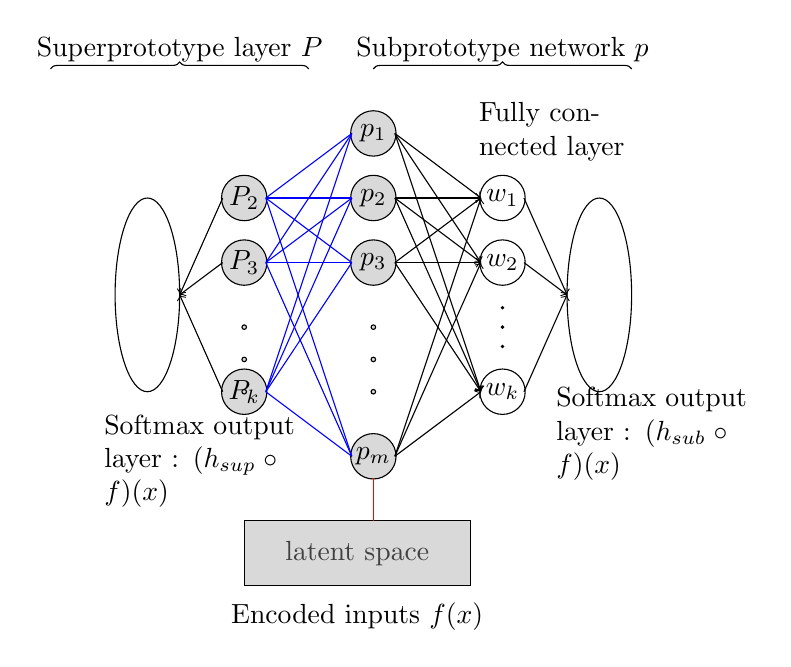
\begin{tikzpicture}[scale=0.82]
\coordinate (p1) at (1,0);
\coordinate (p2) at (1,2);
\coordinate (p3) at (1,3);
\coordinate (p4) at (1,4);
\coordinate (pn) at (1,5);
\coordinate (o1) at (3,1);
\coordinate (o2) at (3,2);
\coordinate (o3) at (3,3);
\coordinate (o4) at (3,4);

\coordinate (sp1) at (-1,1);
\coordinate (sp2) at (-1,2);
\coordinate (sp3) at (-1,3);
\coordinate (sp4) at (-1,4);
\coordinate (spn) at (-1,5);
\coordinate (so1) at (-3,1);
\coordinate (so2) at (-3,2);
\coordinate (so3) at (-3,3);
\coordinate (so4) at (-3,4);
% SUPER
\filldraw[fill=gray!30, draw=black] (sp1) circle (1em) node {$P_k$};
\filldraw[fill=gray!30, draw=black] (sp2) circle (0.1em);
\filldraw[fill=gray!30, draw=black] (-1,1.5) circle (0.1em);
\filldraw[fill=gray!30, draw=black] (-1,1) circle (0.1em);
\filldraw[fill=gray!30, draw=black] (sp3) circle (1em) node {$P_3$};
\filldraw[fill=gray!30, draw=black] (sp4) circle (1em) node {$P_2$};
%\filldraw[fill=gray!30, draw=black] (spn) circle (1em) node {$s_1$}  node[above, yshift=1em, text width=3cm, xshift=1em] {Superprototype layer};
\filldraw[fill=white, draw=black] (-2.5,2.5) ellipse (0.5 and 1.5) node[below,yshift=-4em, text width=2.5cm, xshift=2em] {Softmax output layer : $(h_{\text{sup}}\circ f)(\bm{x})$};
\foreach \j [evaluate=\j as \itext using int(\j)]in {1,3,4}
{
  \path[->] (-1.333, \j) edge (-2, 2.5);
}
\filldraw[fill=gray!30, draw=black] (-1,-1) rectangle (2.5,-2) node[color=darkgray,midway] {latent space} node[color=black, midway, below, yshift=-0.5cm] {Encoded inputs $f(\bm{x})$};

% SUB
\filldraw[fill=gray!30, draw=black] (p1) circle (1em) node {$p_m$};
\filldraw[fill=gray!30, draw=black] (p2) circle (0.1em);
\filldraw[fill=gray!30, draw=black] (1,1.5) circle (0.1em);
\filldraw[fill=gray!30, draw=black] (1,1) circle (0.1em);
\filldraw[fill=gray!30, draw=black] (p3) circle (1em) node {$p_3$};
\filldraw[fill=gray!30, draw=black] (p4) circle (1em) node {$p_2$};
\filldraw[fill=gray!30, draw=black] (pn) circle (1em) node {$p_1$};
\filldraw[fill=white, draw=black] (o1) circle (1em) node {$w_k$};
\filldraw[fill=gray!30, draw=black] (3,2) circle (0.05em);
\filldraw[fill=gray!30, draw=black] (3,2-0.3) circle (0.05em);
\filldraw[fill=gray!30, draw=black] (3,2+0.3) circle (0.05em);
\filldraw[fill=white, draw=black] (o3) circle (1em) node {$w_2$};
\filldraw[fill=white, draw=black] (o4) circle (1em)node {$w_1$} node [above,yshift=1em, text width=2cm, xshift=2em] {Fully connected layer};
 \foreach \i [evaluate=\i as \itext using int(\i)] in {0,3,4,5}
 {
    \foreach \j [evaluate=\j as \itext using int(\j)]in {1,3,4}
    {
      \path[->] (1.333, \i) edge (2.666666666666, \j);
    }
  }
\filldraw[fill=white, draw=black] (4.5,2.5) ellipse (0.5 and 1.5) node[below,yshift=-3em, text width=2.5cm, xshift=2em] {Softmax output layer : $(h_{\text{sub}}\circ f)(\bm{x})$};
  \foreach \j [evaluate=\j as \itext using int(\j)]in {1,3,4}
    {
      \path[->] (3.333, \j) edge (4, 2.5);
    }
 \draw [decorate,decoration={brace}] (1,6) -- (5,6) node[midway,yshift=0.25cm]{Subprototype network $p$};
 \draw [decorate,decoration={brace}] (-4,6) -- (0,6) node[midway,yshift=0.25cm]{Superprototype layer $P$};
 
 \draw [color=red] (1,-1) edge (1,-0.33); 
  \foreach \i [evaluate=\i as \itext using int(\i)] in {0,3,4,5}
 {
    \foreach \j [evaluate=\j as \itext using int(\j)]in {1,3,4}
    {
      \draw[color=blue] (0.6666, \i) edge (-0.666, \j);
    }
  }
\end{tikzpicture}}
